%   ------------------------------------------------------------------------
\FloatBarrier
\section{Análise do God Mode AI}
\label{s.godmodeAI}

A plataforma God Mode AI foi selecionada para a análise devido a seu foco explícito na animação de sprites para jogos. Um aspecto relevante desta ferramenta é seu processo de evolução constante. Durante o período de testes, foram observadas atualizações periódicas na interface e na aplicação, o que resultou em experiências de uso distintas.

Durante os testes, o objetivo principal foi gerar uma animação do personagem Pablo andando. 

Na primeira interação com a ferramenta, havia um setor e procedimento específico para pixel art. O processo consiste em três etapas: \begin{itemize}
    \item O sprite original é convertido para uma versão de alta resolução (Figura \ref{fig:godmodAIpixelto3D} no Apêndice \ref{ap.telasIA}); 
    \item A animação era gerada nesse formato de alta qualidade, com alternativas de direção, movimento e auto reposicionamento (que ajusta o ângulo e a pose da imagem para corresponder ao primeiro quadro da animação), além da possibilidade de usar prompts (Figura \ref{fig:godmodAIGerarAnimacao} no Apêndice \ref{ap.telasIA}); e
    \item A animação resultante era convertida de volta para o estilo pixel art, com opções de personalização de tamanho do pixel e paleta de cores (Figura \ref{fig:godmodAI3Dtopixel} no Apêndice \ref{ap.telasIA}).
\end{itemize}

Os resultados obtidos \footnote{https://drive.google.com/drive/folders/1BKe0jiX1ohblO0YUeFw540fDjaotn8tD?usp=sharing} foram superiores ao de outras ferramentas analisadas na época, conseguindo ser pixel perfect e reconhecendo em geral as características do personagem. Contudo, observou-se uma clara diferença visual entre o sprite original e a animação, pois o estilo de pixel art específico não foi replicado, de forma que o personagem ficava ou muito detalhado ou muito simples, como pode ser visto na Figura \ref{fig:godmodAIComparar}. Além disso, a animação formada exibia o personagem andando na diagonal, inadequada para o cenário side view do jogo 2D, característica que persistiu mesmo após a pixelização.

\begin{figure}[htbp]
    \centering
    \caption{\small Comparação do sprite original com quadros das animações geradas}
    \label{fig:godmodAIComparar}
    \begin{subfigure}{0.21\linewidth}
        
\includegraphics[width=0.6\linewidth]{figs/sprites/Pablo.PNG}
        \caption{\small Imagem de referência}
        \label{fig:godmodAIPablo}
    \end{subfigure}
    \begin{subfigure}{0.21\linewidth}
        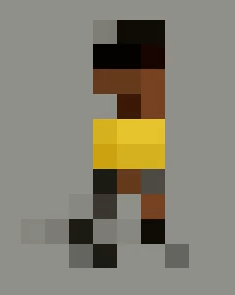
\includegraphics[width=1\linewidth]{figs/godmodAI/print32.PNG}
        \caption{\small Frame da animação de 32 pixels de tamanho}
        \label{fig:godmodAIFrame32}
    \end{subfigure}
    \begin{subfigure}{0.21\linewidth}
        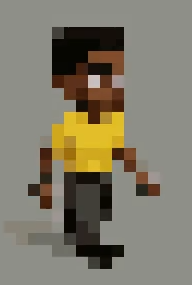
\includegraphics[width=0.85\linewidth]{figs/godmodAI/print64.PNG}
        \caption{\small Frame da animação de 64 pixels de tamanho}
        \label{fig:godmodAIFrame64}
    \end{subfigure}
    \begin{subfigure}{0.21\linewidth}
        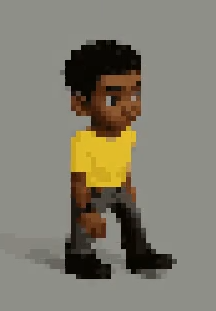
\includegraphics[width=0.88\linewidth]{figs/godmodAI/print152.PNG}
        \caption{\small Frame da animação de 152 pixels de tamanho}
        \label{fig:godmodAIFrame152}
    \end{subfigure}

    \legend{\small Fonte: Elaborada pela autora, utilizando a ferramenta God Mode AI.}
\end{figure}

A análise foi limitada pelo sistema de créditos da plataforma, que disponibilizou apenas três créditos gratuitos (um por etapa), número insuficiente para uma exploração mais aprofundada.

Em uma segunda fase de testes, a interface da ferramenta havia sido modificada, recomendando o uso da funcionalidade principal antes de recorrer ao módulo específico de pixel art (Figura \ref{fig:godmodModificado} no Apêndice \ref{ap.telasIA}), com um crédito adicional disponibilizado. É importante comentar que a ferramenta principal correspondia à segunda etapa da seção de pixel art. A interface também passou a especificar que múltiplas tentativas de reposicionamento não gastam crédito, o que permitiu uma interação mais completa (Figura \ref{fig:godmodAIrepose} no Apêndice \ref{ap.telasIA}) até chegar a um resultado aceitável (Figura \ref{fig:godmodAIreposeFinal}).

\begin{figure}[htbp]
    \centering
    \caption{\small Resultado do auto reposicionamento}
    \label{fig:godmodAIreposeFinal}
    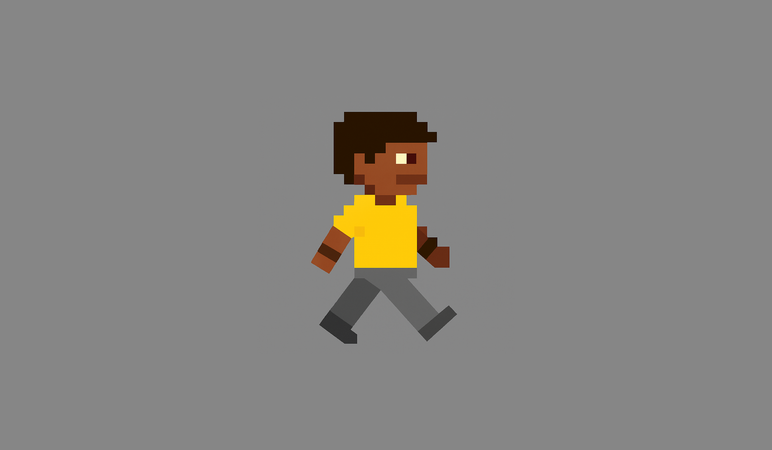
\includegraphics[width=0.5\linewidth]{figs/godmodAI/resultadoRepose.png}
    \legend{\small Fonte: Elaborada pela autora, utilizando a ferramenta God Mode AI.}
\end{figure}

O resultado \footnote{https://drive.google.com/file/d/1uIeHmuF0SmPfPp72ER-hFL9hV-NA0qok/view?usp=sharing} gerado no ambiente principal foi visivelmente superior ao da primeira análise, embora ainda não representasse um personagem exatamente igual ao de referência. Diferente da animação anterior, esta não era pixel perfect, apresentando deformações, como pode ser visto na Figura \ref{fig:godmodAImao}.

\begin{figure}[htbp]
    \centering
    \caption{\small Quadro da animação com a mão deformada no God Mode AI}
    \label{fig:godmodAImao}
    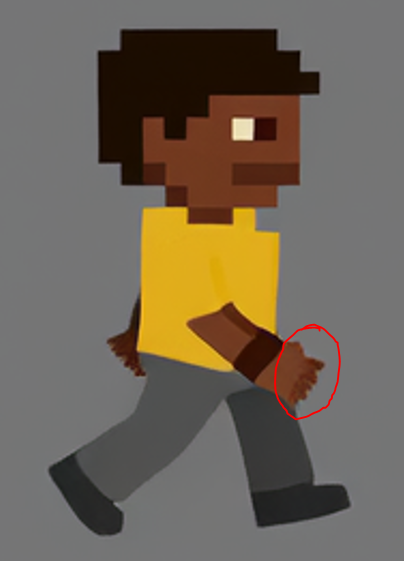
\includegraphics[width=0.3\linewidth]{figs/godmodAI/maoDeformada.PNG}
    \legend{\small Fonte: Elaborada pela autora, utilizando a ferramenta God Mode AI.}
\end{figure}

A principal inovação observada foi a funcionalidade de re-geração parcial (Figura \ref{fig:godmodAIregen}), que permite ao usuário selecionar quadros específicos de uma animação para serem gerados novamente. Este recurso possui grande potencial para o ajuste fino de animações, mas, por custar um crédito, não pôde ser testado.

O God Mode AI demonstrou ser a ferramenta com o desenvolvimento mais ativo e com o maior potencial entre as analisadas até o momento. Funcionalidades como auto reposicionamento e re-geração parcial são diferenciais importantes para uma edição mais rápida da animação formada. Embora ofereça um número limitado de animações, a plataforma permite treinar um novo tipo de movimento no modelo de IA pelo custo de 10 créditos. Outra funcionalidade importante é a exportação da animação como um sprite sheet(Figura \ref{fig:godmodAispriteSheet}), o que facilita seu processo de edição e importação para o Unity. %terceiro acesso site tem opção de sprite sheet transparente, mas quando fui testar deu erro.

\begin{figure}[htbp]
    \centering
    \caption{\small Sprite sheet do resultado final no God Mode AI}
    \label{fig:godmodAispriteSheet}
    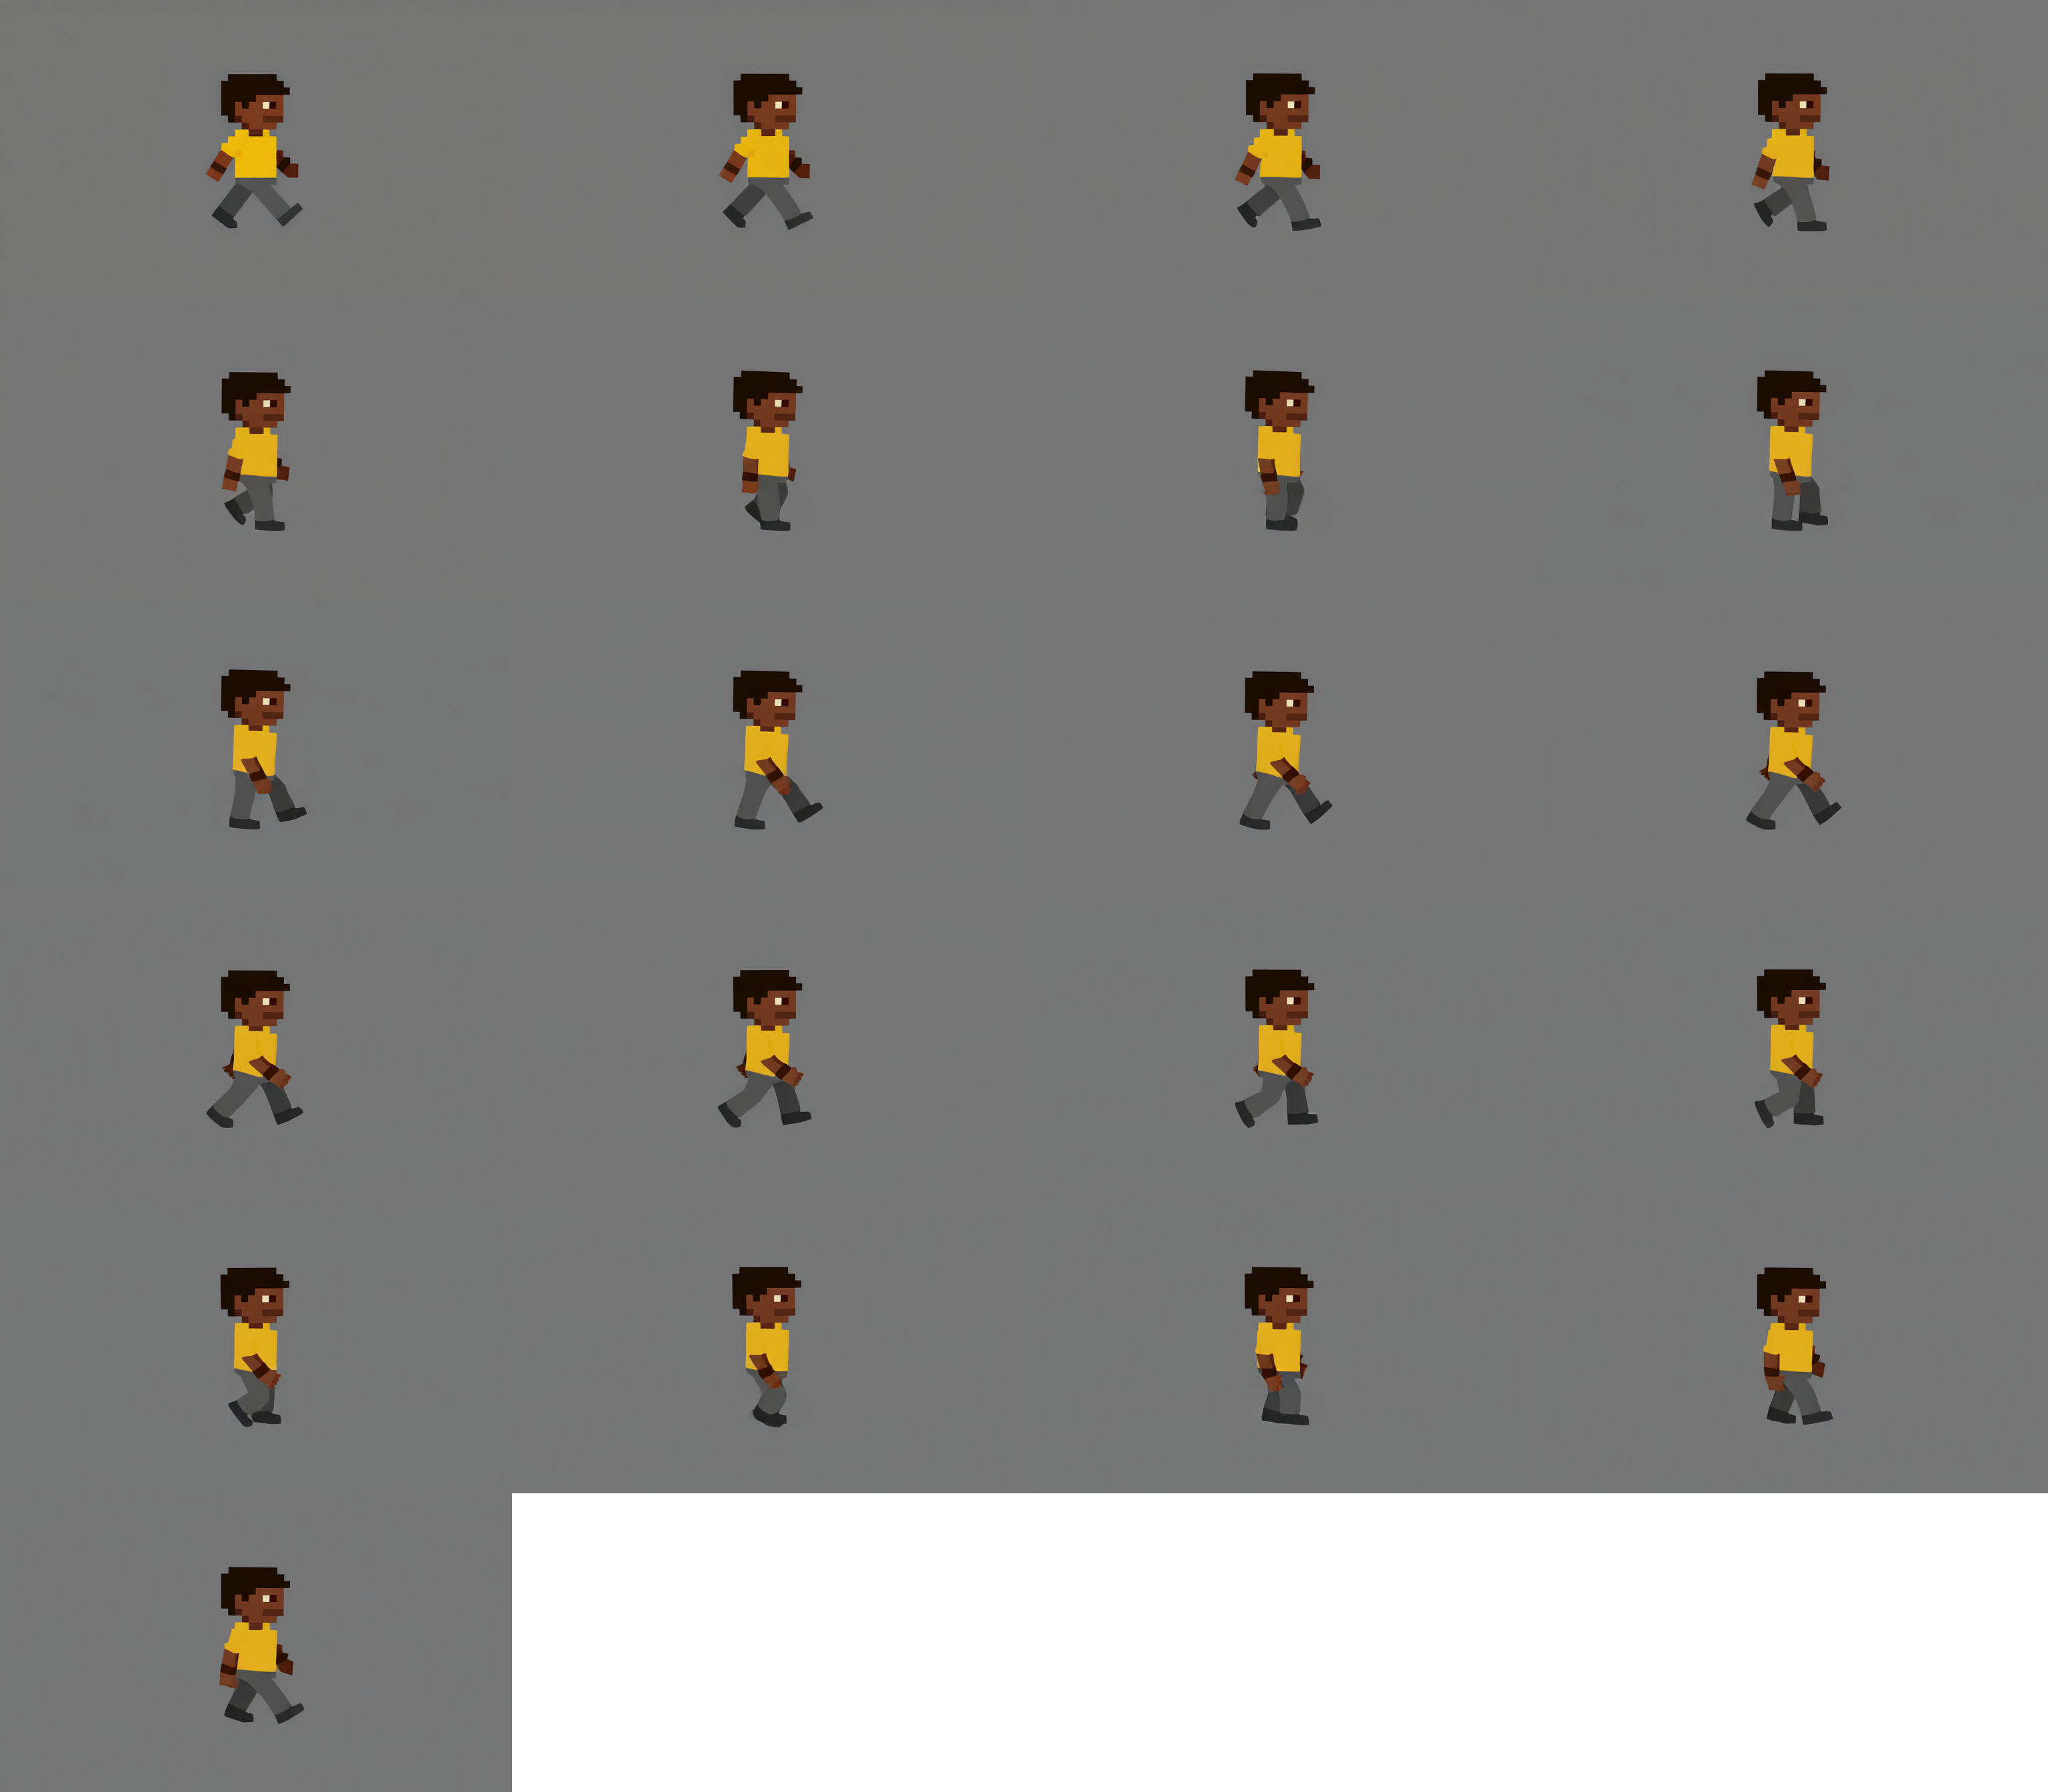
\includegraphics[width=1\linewidth]{figs/godmodAI/sprite sheet.png}
    \legend{\small Fonte: Elaborada pela autora, utilizando a ferramenta God Mode AI.}
\end{figure}

Apesar do potencial, devido à limitação de créditos, os resultados dos testes não atingiram a consistência e a qualidade necessárias para a aplicação direta no jogo. No entanto, o sprite sheet gerado nesta etapa servirá como referência para a análise da ferramenta Pixel Lab (detalhada na Seção \ref{s.pixelLab.animacao}), tendo que ser convertido para o padrão pixel perfect através do Pixilart\footnote{https://www.pixilart.com/draw?ref=home-page} (plataforma online para desenhar no estilo pixel art, abrindo qualquer imagem e permitindo a redimensão do conteúdo da mesma em pixels). Na Figura \ref{fig:godmodAispriteSheetPixel} pode ser verificado o resultado dessa conversão.

\begin{figure}[htbp]
    \centering
    \caption{\small Sprite sheet convertido para pixel art}
    \label{fig:godmodAispriteSheetPixel}
    
\includegraphics[width=1\linewidth]{figs/godmodAI/Pixilart/pixilart-sprite.png}
    \legend{\small Fonte: Elaborada pela autora, utilizando a ferramenta Pixilart.}
\end{figure}



